%%%%%%%%%%%%%%%%%%%%%%%%%%%%%%%%%%%%%%%%%%%%%%%%%%%%%%%%%%%%
%%  This Beamer template was created by Cameron Bracken.
%%  Anyone can freely use or modify it for any purpose
%%  without attribution.
%%
%%  Last Modified: January 9, 2009
%%

\documentclass[xcolor=x11names,compress]{beamer}

%% General document %%%%%%%%%%%%%%%%%%%%%%%%%%%%%%%%%%
\usepackage{graphicx}
\usepackage{tikz}
\usetikzlibrary{lindenmayersystems}
\usepackage[utf8]{inputenc}
\usepackage{verbatim}
\usepackage{fancyvrb}
\usepackage{pifont}
\usepackage{mathrsfs}
\usepackage{pmboxdraw}
\usepackage{minted}
%%%%%%%%%%%%%%%%%%%%%%%%%%%%%%%%%%%%%%%%%%%%%%%%%%%%%%
% Code snippets
\newminted{python}{fontsize=\scriptsize, 
		   framesep=3mm}

%% Beamer Layout %%%%%%%%%%%%%%%%%%%%%%%%%%%%%%%%%%
\useoutertheme[subsection=false,shadow]{miniframes}
\useinnertheme{default}
\usefonttheme{serif}
\usepackage{palatino}

\setbeamerfont{title like}{shape=\scshape}
\setbeamerfont{frametitle}{shape=\scshape}

\setbeamercolor*{lower separation line head}{bg=DeepSkyBlue4}
\setbeamercolor*{normal text}{fg=black,bg=white}
\setbeamercolor*{alerted text}{fg=red}
\setbeamercolor*{example text}{fg=black}
\setbeamercolor*{structure}{fg=black}

\setbeamercolor*{palette tertiary}{fg=black,bg=black!10}
\setbeamercolor*{palette quaternary}{fg=black,bg=black!10}

\renewcommand{\(}{\begin{columns}}
\renewcommand{\)}{\end{columns}}
\newcommand{\<}[1]{\begin{column}{#1}}
\renewcommand{\>}{\end{column}}
%%%%%%%%%%%%%%%%%%%%%%%%%%%%%%%%%%%%%%%%%%%%%%%%%%
\setbeamertemplate{caption}[numbered]       % Numbered figures
\setbeamertemplate{navigation symbols}{}    % No navigation footer
%\setbeamertemplate{footline}[page number]

\begin{document}

% Code snippets
\defverbatim[colored]\codeFactorial{
\begin{pythoncode}
def factorial(n):
    """
    Returns the factorial of n
    (int -> int)

    >>> factorial(2)
    2
    >>> factorial(3)
    6
    """
    if n:
        return n*factorial(n-1)
    else:
        return 1
\end{pythoncode}
}

\defverbatim[colored]\codeFactorialTarget{
\begin{pythoncode*}{fontsize=\huge}
@UTBP
def factorial(n):
    """
    factorial(0) == 1
    factorial(1) == 1
    factorial(2) == 2
    factorial(3) == 6
    """
\end{pythoncode*}
}

\defverbatim[colored]\codeLengthIteration{
\begin{pythoncode*}{fontsize=\large}
def length(l):
    i = 0
    for e in l:
        i += 1
    return i
\end{pythoncode*}
}

\defverbatim[colored]\codeLengthRecursion{
\begin{pythoncode*}{fontsize=\large}
def length(l):
    if l:
        return length(l[1:])+1
    else:
        return 0
\end{pythoncode*}
}

\defverbatim[colored]\codeLengthRecursionSmall{
\begin{pythoncode*}{fontsize=\scriptsize}
def length(l):
    if l: return 1+length(l[1:])
    else: return 0
\end{pythoncode*}
}

\defverbatim[colored]\codeLengthExampleA{
\begin{pythoncode*}{fontsize=\large}
@UTBP
def length(l):
"""
length(()) == 0
"""
\end{pythoncode*}
}

\defverbatim[colored]\codeLengthExampleB{
\begin{pythoncode*}{fontsize=\large}
@UTBP
def length(l):
"""
length(()) == 0
length((2,)) == 1
"""
\end{pythoncode*}
}

\defverbatim[colored]\codeLengthExampleC{
\begin{pythoncode*}{fontsize=\Large}
@UTBP
def length(l):
"""
length(()) == 0
length((2,)) == 1
length((2, 3)) == 2
"""
\end{pythoncode*}
}

\defverbatim[colored]\codeImpossible{
\begin{pythoncode*}{fontsize=\scriptsize}
@UTBP
def impossible(l):
"""
impossible(0) == 0
impossible(0) == 1
"""
\end{pythoncode*}
}


%%%%%%%%%%%%%%%%%%%%%%%%%%%%%%%%%%%%%%%%%%%%%%%%%%%%%%
%%%%%%%%%%%%%%%%%%%%%%%%%%%%%%%%%%%%%%%%%%%%%%%%%%%%%%
\begin{frame}
    \title{Programación basada en pruebas unitarias}
\author{Miguel Lechón} 
\date{28 de diciembre de 2014}
\titlepage
\end{frame}

%%%%%%%%%%%%%%%%%%%%%%%%%%%%%%%%%%%%%%%%%%%%%%%%%%%%%%
%%%%%%%%%%%%%%%%%%%%%%%%%%%%%%%%%%%%%%%%%%%%%%%%%%%%%%
%\section*{\scshape Outline}
%\begin{frame}{Outline of the presentation}
%\tableofcontents[hideallsubsections]
%\end{frame}

%%%%%%%%%%%%%%%%%%%%%%%%%%%%%%%%%%%%%%%%%%%%%%%%%%%%%%
%%%%%%%%%%%%%%%%%%%%%%%%%%%%%%%%%%%%%%%%%%%%%%%%%%%%%%
\section{\scshape Introducción}
\subsection{SIGBOVIK}
\begin{frame}{Contexto -- SigBOVIK}
    \begin{figure}[t]
        \centering
        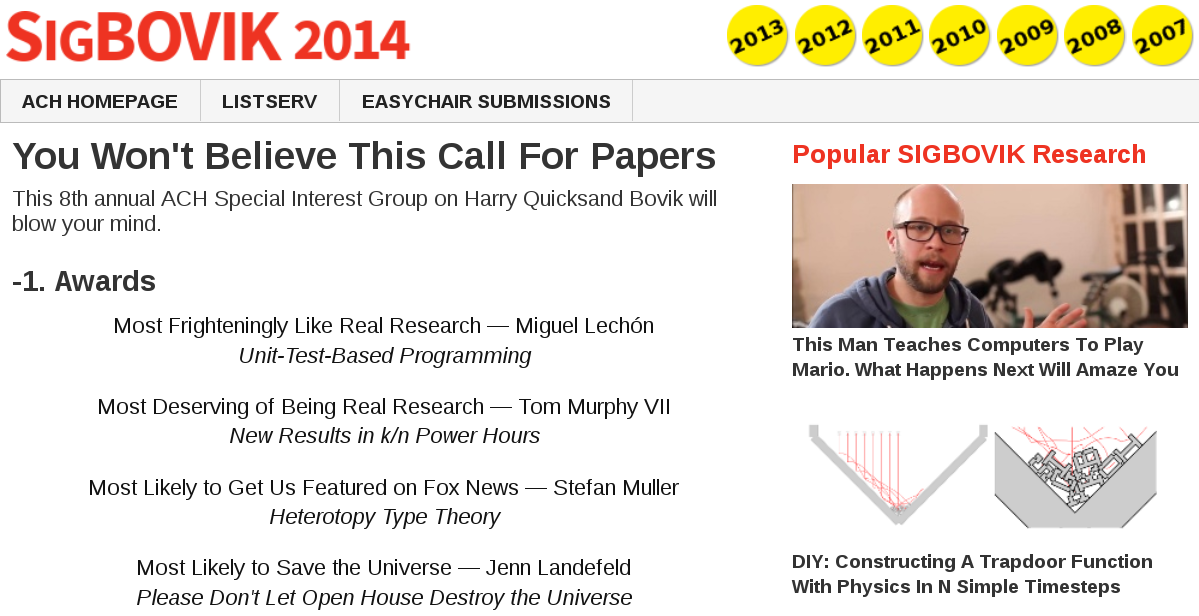
\includegraphics[width=1.0\textwidth]{images/sigbovik.png}
    \end{figure}
\end{frame}

%%%%%%%%%%%%%%%%%%%%%%%%%%%%%%%%%%%%%%%%%%%%%%%%%%%%%%
%%%%%%%%%%%%%%%%%%%%%%%%%%%%%%%%%%%%%%%%%%%%%%%%%%%%%%
\subsection{Yo}
\begin{frame}{Yo}
    \frametitle{Contexto -- Yo}
    \begin{itemize}
        \item Informático \pause
        \item Programador \textcolor{red}{sin código en producción} \pause
        \item Administrador de sistemas \textcolor{red}{mediocre} \pause
        \item Ex-estudiante de doctorado \textcolor{red}{sin doctorado} \pause
        \item Actualmente, \textcolor{blue}{ama de casa}
    \end{itemize}
\end{frame}

%%%%%%%%%%%%%%%%%%%%%%%%%%%%%%%%%%%%%%%%%%%%%%%%%%%%%%
%%%%%%%%%%%%%%%%%%%%%%%%%%%%%%%%%%%%%%%%%%%%%%%%%%%%%%
\subsection{Motivación}
\begin{frame}{Motivación}
    ¿En qué consiste programar?
    \begin{columns}
        \begin{column}{.5\linewidth}
        \begin{block}
            \codeFactorial
        \end{block}
        \end{column}
        \begin{column}{.5\linewidth}
            \begin{itemize}\itemsep25pt \pause
                \item Explicar qué se espera del código\pause
                \item Explicarlo otra vez, por si las moscas\pause
                \item Explicarlo de nuevo, esta vez para el ordenador\pause
            \end{itemize}
        \end{column}
    \end{columns}
    Uno no aprende a programar para trabajar más de la cuenta.
\end{frame}

%%%%%%%%%%%%%%%%%%%%%%%%%%%%%%%%%%%%%%%%%%%%%%%%%%%%%%
%%%%%%%%%%%%%%%%%%%%%%%%%%%%%%%%%%%%%%%%%%%%%%%%%%%%%%
\subsection{Objetivo}
\begin{frame}{Objetivo}
    \pause
    \codeFactorialTarget
\end{frame}


%%%%%%%%%%%%%%%%%%%%%%%%%%%%%%%%%%%%%%%%%%%%%%%%%%%%%%
%%%%%%%%%%%%%%%%%%%%%%%%%%%%%%%%%%%%%%%%%%%%%%%%%%%%%%
\subsection{Pero\ldots ¿cómo?}
\begin{frame}{Pero\ldots ¿cómo?}
    Premisas:
    \pause
    \begin{itemize}
        \item Toda función se puede escribir de forma recursiva \pause
        \item Toda función recursiva puede representarse mediante un árbol \pause
        \item Los árboles se pueden enumerar en order creciente de complejidad \pause
    \end{itemize}
    Conclusión:

    \textbf{$\rightarrow$ Podemos enumerar todas las funciones de forma ordenada} \pause

    (y comprobar, una a una, si satisfacen nuestras pruebas unitarias)
\end{frame}

%%%%%%%%%%%%%%%%%%%%%%%%%%%%%%%%%%%%%%%%%%%%%%%%%%%%%%
%%%%%%%%%%%%%%%%%%%%%%%%%%%%%%%%%%%%%%%%%%%%%%%%%%%%%%

\section{\scshape Premisas}

\subsection{Toda función se puede escribir de forma recursiva}
\begin{frame}{Funciones: todas recursivas}
    \textcolor{red}{Advertencia:} Este es un ejercicio académico \pause extremadamente complejo\pause. Gritad si os perdéis. \pause
    \begin{columns}
        \begin{column}{.30\linewidth}
        \begin{block}
            \codeLengthIteration
        \end{block}
        \end{column}
        \begin{column}{.65\linewidth}
        \begin{block}
            \codeLengthRecursion
        \end{block}
        \end{column}
    \end{columns} \pause
    La versión recursiva es claramente superior.
\end{frame}

%%%%%%%%%%%%%%%%%%%%%%%%%%%%%%%%%%%%%%%%%%%%%%%%%%%%%%
%%%%%%%%%%%%%%%%%%%%%%%%%%%%%%%%%%%%%%%%%%%%%%%%%%%%%%

\subsection{Expresiones como árboles}
\begin{frame}[fragile]
    \frametitle{Expresiones como árboles}
    $$\frac{-b\pm\sqrt{b^2-4ac}}{2a}$$

\begin{Verbatim}[commandchars=\\\{\},codes={\catcode`$=3\catcode`_=8}]
        \textbf{/}
        ├── \textbf{+/-}
        │   ├── \textbf{neg}
        │   │   └── b
        │   └── \textbf{sqrt}
        │       └── \textbf{-}
        │           ├── \textbf{^}
        │           │   ├── b
        │           │   └── 2
        │           └── \textbf{*}
        │               ├── 4
        └── \textbf{*}           └── \textbf{*}
            ├── 2           ├── a
            └── a           └── c
\end{Verbatim}
\end{frame}



\subsection{Toda función recursiva puede representarse mediante un árbol}
\begin{frame}[fragile]
    \frametitle{Funciones recursivas: todas árboles}
    \codeLengthRecursionSmall
\begin{Verbatim}[commandchars=\\\{\},codes={\catcode`$=3\catcode`_=8}]
\textbf{python}                \textbf{pseudo-scheme}
def                   define                    
  length              ├── length                
                      └── lambda                
(l):                      ├── l                 
    if                    └── if                
      l:                      ├── l             
        return 1+             ├── succ          
            length(           │   └── length    
                l[1:]         │       └── cdr   
            )                 │           └── l 
    else: return 0            └── 0             
\end{Verbatim}
\end{frame}

\subsection{Los árboles se pueden enumerar en order creciente de complejidad \pause}
\begin{frame}[fragile]
    \frametitle{Árboles: enumerables}
\begin{Verbatim}[commandchars=\\\{\},codes={\catcode`$=3\catcode`_=8}]
     [\textbf{1}]   [  \textbf{2}  ]    [        \textbf{3}       ]
      r     r          r         r
            └── l      └── b     ├── l0
                           └── l └── l1
\end{Verbatim}

\pause

\begin{Verbatim}[commandchars=\\\{\},codes={\catcode`$=3\catcode`_=8}]
     [               \textbf{4}                 ]
      r          r          r         
      └── b0     └── b0     ├── b0    
          └── b1     ├── l0 │   └── l0
              └── l0 └── l1 └── l1    
            r             r
            ├── b0        ├── l0
            └── b1        ├── l1
                └── l0    └── l2
\end{Verbatim}



\end{frame}

\section{\scshape Ingredientes}
\subsection{Ingredientes}
\begin{frame}{Ingredientes}
    \begin{itemize}
        \item Árboles \pause \emph{(déjà vu)} \pause \textcolor{gray}{\scriptsize(de jabugo)} \pause
        \item Tipos: \pause
            \begin{itemize}
            \item Números naturales no negativos \pause
            \item Listas, posiblemente anidadas \pause
            \end{itemize}
        \item Operaciones: \pause
            \begin{itemize}
                \item Funciones aritméticas (e.g. \texttt{succ}) \pause
                \item Manipulación de listas (e.g. \texttt{cdr}) \pause
                \item Formas especiales (\texttt{if}) \pause
            \end{itemize}
        \item Constantes (operaciones sobre cero elementos): \pause
            \begin{itemize}
                \item \texttt{0} \pause
                \item \texttt{()}
            \end{itemize}
    \end{itemize}
\end{frame}

\section{\scshape Ejemplo de uso}
\subsection{Ejemplo}
\begin{frame}[fragile]
    \frametitle{Ejemplo de uso -- Longitud de una lista}\pause
    \begin{columns}
        \begin{column}{.50\linewidth}
        \begin{block}
            \codeLengthExampleA
        \end{block}
        \end{column}\pause
        \begin{column}{.50\linewidth}
        \begin{verbatim}
define
├── length
└── lambda
    ├── l
    └── 0
        \end{verbatim}
        \end{column}
    \end{columns}\pause

    \begin{columns}
        \begin{column}{.50\linewidth}
        \begin{block}
            \codeLengthExampleB
        \end{block}
        \end{column}\pause
        \begin{column}{.50\linewidth}
        \begin{verbatim}
define
├── length
└── lambda
    ├── l
    └── if
        ├── l
        ├── list?
        │   └── l
        └── 0
        \end{verbatim}
        \end{column}
    \end{columns}
\end{frame}

%%%%%%%%%%%%%%%%%%%%%%%%%%%%%%%%%%%%%%%%%%%%%%%%%%%%%%
%%%%%%%%%%%%%%%%%%%%%%%%%%%%%%%%%%%%%%%%%%%%%%%%%%%%%%

\subsection{Ejemplo}
\begin{frame}[fragile]
    \frametitle{Ejemplo de uso -- Longitud de una lista}
    \begin{columns}
        \begin{column}{.50\linewidth}
        \begin{block}
            \codeLengthExampleC
        \end{block}
        \end{column}\pause
        \begin{column}{.50\linewidth}
        \begin{verbatim}
define
├── length
└── lambda
    ├── l
    └── if
        ├── l
        ├── succ
        │   └── length
        │       └── cdr
        │           └── l
        └── 0
        \end{verbatim}
        \end{column}
    \end{columns}
\end{frame}

%%%%%%%%%%%%%%%%%%%%%%%%%%%%%%%%%%%%%%%%%%%%%%%%%%%%%%
%%%%%%%%%%%%%%%%%%%%%%%%%%%%%%%%%%%%%%%%%%%%%%%%%%%%%%
\section{\scshape Propiedades}
\subsection{Propiedades}
\begin{frame}{Propiedades}
    \begin{itemize}
        \item Corrección garantizada
            \begin{block}
                \codeImpossible
            \end{block}
    \end{itemize}
\end{frame}

\end{document}
